\documentclass{standalone}
\usepackage{tikz}
\usetikzlibrary{patterns, positioning}
\usepackage[sfdefault]{ClearSans} %% option 'sfdefault' activates Clear Sans as the default text font
\usepackage[T1]{fontenc}

\begin{document}
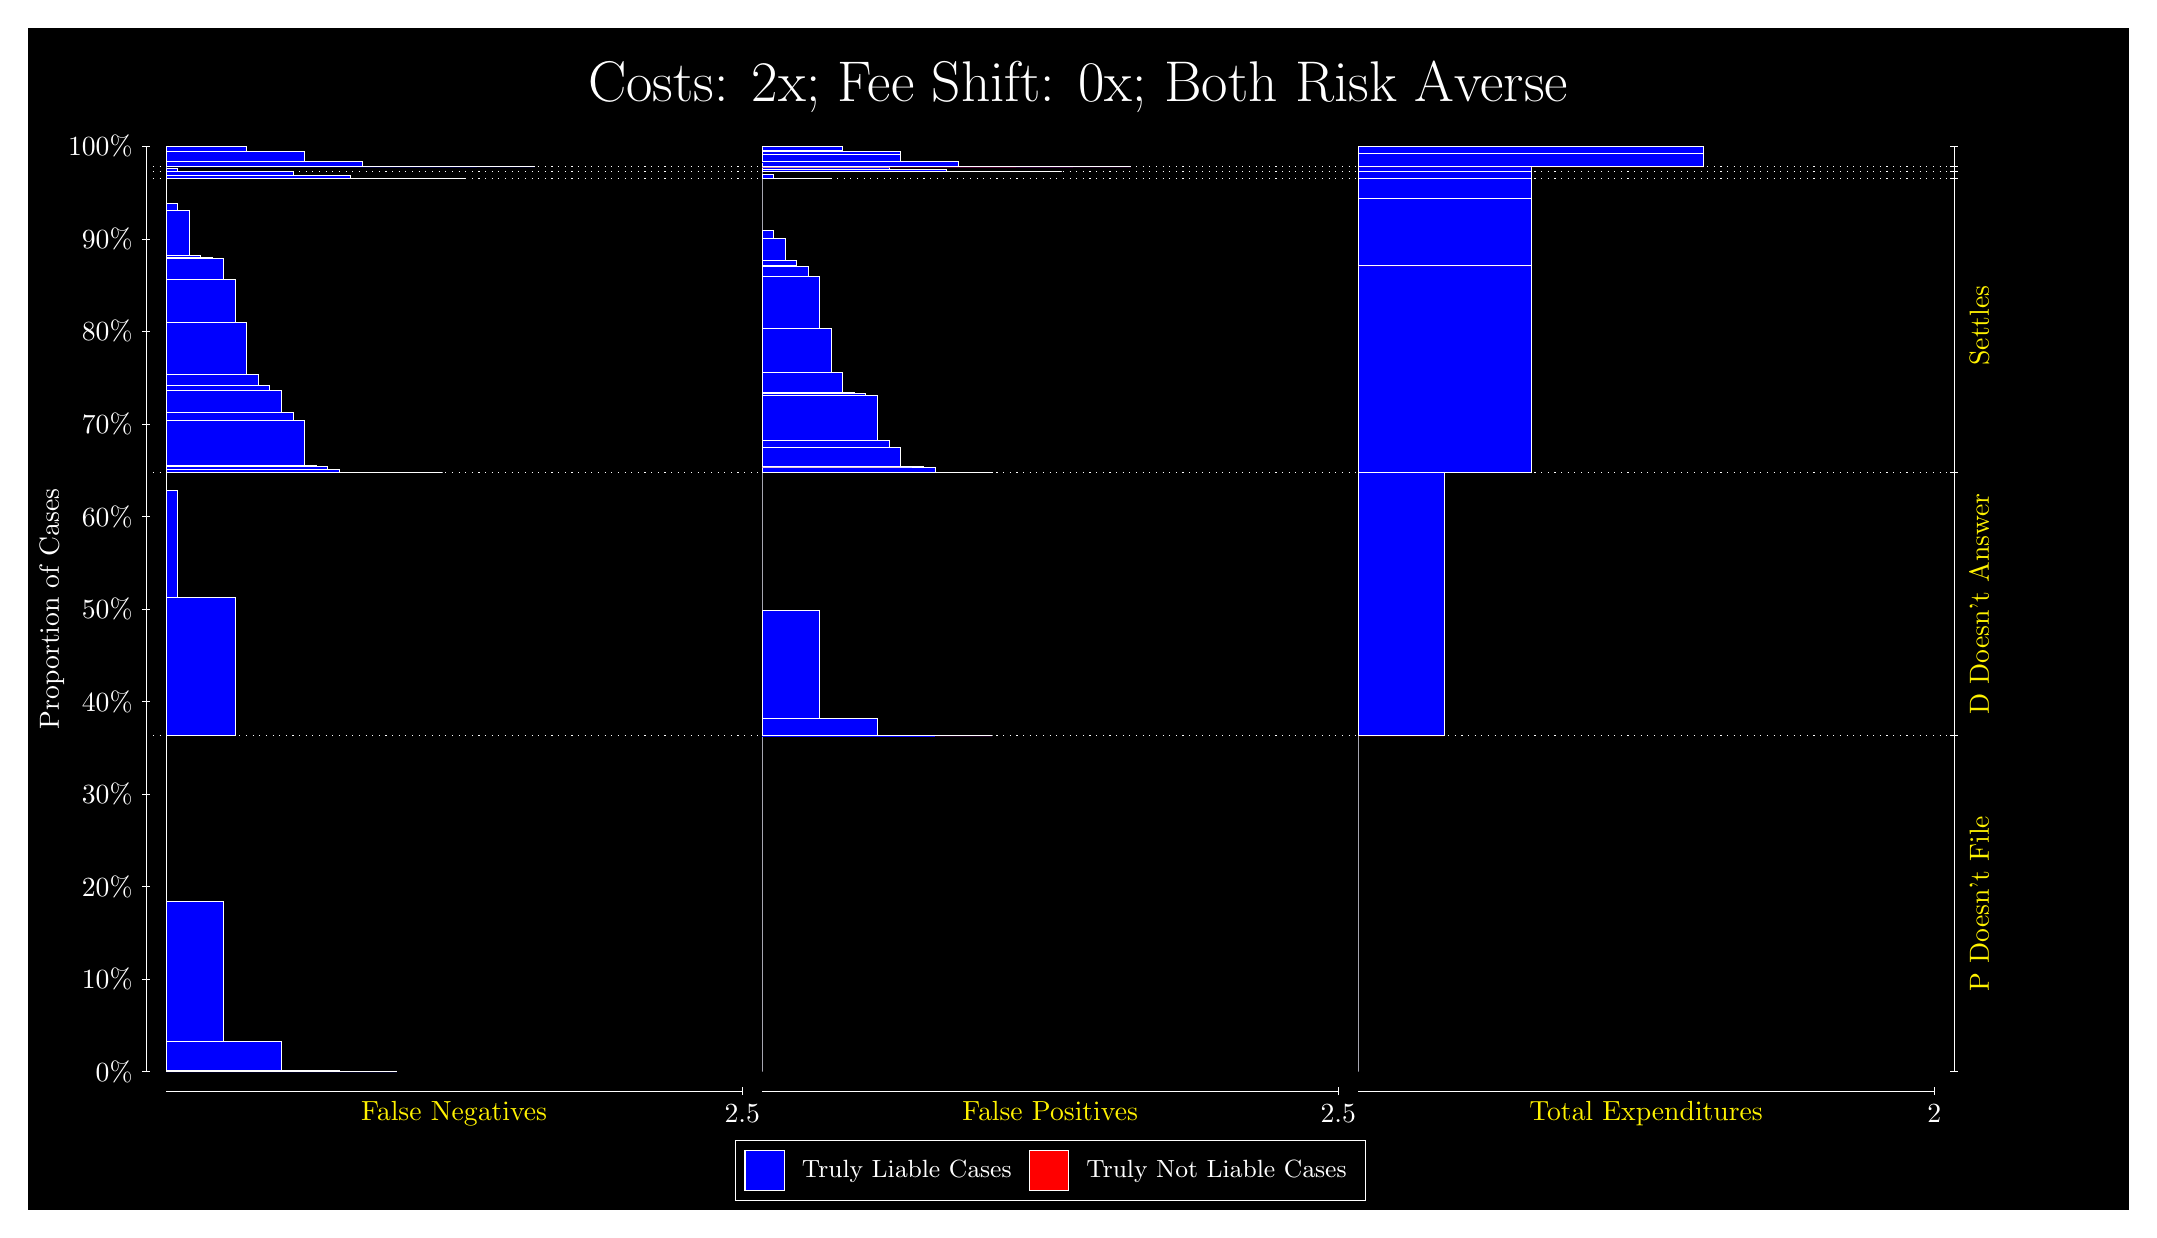
\begin{tikzpicture}
\draw[fill=black] (0,0) rectangle (26.667,15);
\draw[text=white] (0,13.5) rectangle (26.667,15) node[midway] {\huge Costs: 2x; Fee Shift: 0x; Both Risk Averse};
\draw[white, very thin] (1.5,1.75) -- (1.5,13.5);
\node[rotate=90, text=white, anchor=center] at (0.3, 7.625) {Proportion of Cases};
\draw[white, very thin] (1.45,1.75) -- (1.55,1.75);
\node[text=white, anchor=east] at (1.45, 1.75) {0\%};
\draw[white, very thin] (1.45,2.925) -- (1.55,2.925);
\node[text=white, anchor=east] at (1.45, 2.925) {10\%};
\draw[white, very thin] (1.45,4.1) -- (1.55,4.1);
\node[text=white, anchor=east] at (1.45, 4.1) {20\%};
\draw[white, very thin] (1.45,5.275) -- (1.55,5.275);
\node[text=white, anchor=east] at (1.45, 5.275) {30\%};
\draw[white, very thin] (1.45,6.45) -- (1.55,6.45);
\node[text=white, anchor=east] at (1.45, 6.45) {40\%};
\draw[white, very thin] (1.45,7.625) -- (1.55,7.625);
\node[text=white, anchor=east] at (1.45, 7.625) {50\%};
\draw[white, very thin] (1.45,8.8) -- (1.55,8.8);
\node[text=white, anchor=east] at (1.45, 8.8) {60\%};
\draw[white, very thin] (1.45,9.975) -- (1.55,9.975);
\node[text=white, anchor=east] at (1.45, 9.975) {70\%};
\draw[white, very thin] (1.45,11.15) -- (1.55,11.15);
\node[text=white, anchor=east] at (1.45, 11.15) {80\%};
\draw[white, very thin] (1.45,12.325) -- (1.55,12.325);
\node[text=white, anchor=east] at (1.45, 12.325) {90\%};
\draw[white, very thin] (1.45,13.5) -- (1.55,13.5);
\node[text=white, anchor=east] at (1.45, 13.5) {100\%};

\draw[white, very thin] (24.457,1.75) -- (24.457,13.5);
\draw[white, very thin] (24.407,1.75) -- (24.507,1.75);
\node[anchor=west] at (24.407, 1.75) {};
\draw[white, very thin] (24.407,6.0148) -- (24.507,6.0148);
\node[anchor=west] at (24.407, 6.0148) {};
\draw[white, very thin] (24.407,9.358) -- (24.507,9.358);
\node[anchor=west] at (24.407, 9.358) {};
\draw[white, very thin] (24.407,13.094) -- (24.507,13.094);
\node[anchor=west] at (24.407, 13.094) {};
\draw[white, very thin] (24.407,13.182) -- (24.507,13.182);
\node[anchor=west] at (24.407, 13.182) {};
\draw[white, very thin] (24.407,13.241) -- (24.507,13.241);
\node[anchor=west] at (24.407, 13.241) {};
\draw[white, very thin] (24.407,13.5) -- (24.507,13.5);
\node[anchor=west] at (24.407, 13.5) {};

\draw[white, very thin, fill=blue] (1.75,1.75) rectangle (4.6775,1.7501);
\draw[white, very thin, fill=blue] (1.75,1.7501) rectangle (3.9457,1.7625);
\draw[white, very thin, fill=blue] (1.75,1.7625) rectangle (3.2138,2.1373);
\draw[white, very thin, fill=blue] (1.75,2.1373) rectangle (2.4819,3.9155);
\draw[white, very thin, fill=red] (1.75,3.9155) rectangle (1.75,3.9155);
\draw[white, very thin, fill=blue] (1.75,3.9155) rectangle (1.75,6.0148);
\draw[white, very thin, fill=blue] (1.75,6.0148) rectangle (2.6283,7.7709);
\draw[white, very thin, fill=blue] (1.75,7.7709) rectangle (1.8964,9.1329);
\draw[white, very thin, fill=red] (1.75,9.1329) rectangle (1.75,9.1329);
\draw[white, very thin, fill=blue] (1.75,9.1329) rectangle (1.75,9.358);
\draw[white, very thin, fill=blue] (1.75,9.358) rectangle (5.2631,9.358);
\draw[white, very thin, fill=blue] (1.75,9.358) rectangle (4.6775,9.3581);
\draw[white, very thin, fill=blue] (1.75,9.3581) rectangle (4.5312,9.3592);
\draw[white, very thin, fill=blue] (1.75,9.3592) rectangle (4.3848,9.3592);
\draw[white, very thin, fill=blue] (1.75,9.3592) rectangle (4.092,9.3594);
\draw[white, very thin, fill=blue] (1.75,9.3594) rectangle (3.9457,9.3952);
\draw[white, very thin, fill=blue] (1.75,9.3952) rectangle (3.7993,9.4382);
\draw[white, very thin, fill=blue] (1.75,9.4382) rectangle (3.6529,9.4444);
\draw[white, very thin, fill=blue] (1.75,9.4444) rectangle (3.5065,10.02);
\draw[white, very thin, fill=blue] (1.75,10.02) rectangle (3.3602,10.121);
\draw[white, very thin, fill=blue] (1.75,10.121) rectangle (3.2138,10.397);
\draw[white, very thin, fill=blue] (1.75,10.397) rectangle (3.0674,10.461);
\draw[white, very thin, fill=blue] (1.75,10.461) rectangle (3.0674,10.47);
\draw[white, very thin, fill=blue] (1.75,10.47) rectangle (2.921,10.599);
\draw[white, very thin, fill=blue] (1.75,10.599) rectangle (2.7746,11.263);
\draw[white, very thin, fill=blue] (1.75,11.263) rectangle (2.6283,11.815);
\draw[white, very thin, fill=blue] (1.75,11.815) rectangle (2.4819,12.075);
\draw[white, very thin, fill=blue] (1.75,12.075) rectangle (2.3355,12.091);
\draw[white, very thin, fill=blue] (1.75,12.091) rectangle (2.3355,12.091);
\draw[white, very thin, fill=blue] (1.75,12.091) rectangle (2.1891,12.113);
\draw[white, very thin, fill=blue] (1.75,12.113) rectangle (2.0428,12.691);
\draw[white, very thin, fill=blue] (1.75,12.691) rectangle (1.8964,12.774);
\draw[white, very thin, fill=red] (1.75,12.774) rectangle (1.75,12.774);
\draw[white, very thin, fill=blue] (1.75,12.774) rectangle (1.75,13.094);
\draw[white, very thin, fill=blue] (1.75,13.094) rectangle (5.5558,13.094);
\draw[white, very thin, fill=blue] (1.75,13.094) rectangle (4.8239,13.094);
\draw[white, very thin, fill=blue] (1.75,13.094) rectangle (4.092,13.127);
\draw[white, very thin, fill=blue] (1.75,13.127) rectangle (3.3602,13.181);
\draw[white, very thin, fill=blue] (1.75,13.181) rectangle (2.6283,13.182);
\draw[white, very thin, fill=red] (1.75,13.182) rectangle (1.75,13.182);
\draw[white, very thin, fill=blue] (1.75,13.182) rectangle (2.6283,13.183);
\draw[white, very thin, fill=blue] (1.75,13.183) rectangle (1.8964,13.219);
\draw[white, very thin, fill=red] (1.75,13.219) rectangle (1.75,13.219);
\draw[white, very thin, fill=blue] (1.75,13.219) rectangle (1.75,13.241);
\draw[white, very thin, fill=blue] (1.75,13.241) rectangle (6.4341,13.241);
\draw[white, very thin, fill=blue] (1.75,13.241) rectangle (5.7022,13.241);
\draw[white, very thin, fill=blue] (1.75,13.241) rectangle (4.9703,13.246);
\draw[white, very thin, fill=blue] (1.75,13.246) rectangle (4.2384,13.306);
\draw[white, very thin, fill=blue] (1.75,13.306) rectangle (3.5065,13.436);
\draw[white, very thin, fill=blue] (1.75,13.436) rectangle (2.7746,13.496);
\draw[white, very thin, fill=blue] (1.75,13.496) rectangle (2.0428,13.5);
\draw[white, very thin, fill=red] (1.75,13.5) rectangle (1.75,13.5);
\draw[white, very thin, fill=blue] (1.75,13.5) rectangle (1.75,13.5);
\draw[white, very thin, fill=red] (9.3189,1.75) rectangle (9.3189,1.75);
\draw[white, very thin, fill=blue] (9.3189,1.75) rectangle (9.3189,6.0148);
\draw[white, very thin, fill=red] (9.3189,6.0148) rectangle (12.246,6.0148);
\draw[white, very thin, fill=blue] (9.3189,6.0148) rectangle (12.246,6.0148);
\draw[white, very thin, fill=blue] (9.3189,6.0148) rectangle (11.515,6.0159);
\draw[white, very thin, fill=blue] (9.3189,6.0159) rectangle (10.783,6.2399);
\draw[white, very thin, fill=blue] (9.3189,6.2399) rectangle (10.051,7.6019);
\draw[white, very thin, fill=blue] (9.3189,7.6019) rectangle (9.3189,9.358);
\draw[white, very thin, fill=red] (9.3189,9.358) rectangle (12.246,9.358);
\draw[white, very thin, fill=blue] (9.3189,9.358) rectangle (12.246,9.3581);
\draw[white, very thin, fill=red] (9.3189,9.3581) rectangle (11.954,9.3581);
\draw[white, very thin, fill=blue] (9.3189,9.3581) rectangle (11.954,9.3581);
\draw[white, very thin, fill=red] (9.3189,9.3581) rectangle (11.661,9.3581);
\draw[white, very thin, fill=blue] (9.3189,9.3581) rectangle (11.661,9.3583);
\draw[white, very thin, fill=blue] (9.3189,9.3583) rectangle (11.515,9.4301);
\draw[white, very thin, fill=red] (9.3189,9.4301) rectangle (11.368,9.4301);
\draw[white, very thin, fill=blue] (9.3189,9.4301) rectangle (11.368,9.4303);
\draw[white, very thin, fill=blue] (9.3189,9.4303) rectangle (11.222,9.4303);
\draw[white, very thin, fill=red] (9.3189,9.4303) rectangle (11.075,9.4303);
\draw[white, very thin, fill=blue] (9.3189,9.4303) rectangle (11.075,9.6775);
\draw[white, very thin, fill=blue] (9.3189,9.6775) rectangle (10.929,9.7609);
\draw[white, very thin, fill=blue] (9.3189,9.7609) rectangle (10.783,10.338);
\draw[white, very thin, fill=blue] (9.3189,10.338) rectangle (10.636,10.361);
\draw[white, very thin, fill=red] (9.3189,10.361) rectangle (10.49,10.361);
\draw[white, very thin, fill=blue] (9.3189,10.361) rectangle (10.49,10.361);
\draw[white, very thin, fill=blue] (9.3189,10.361) rectangle (10.49,10.376);
\draw[white, very thin, fill=blue] (9.3189,10.376) rectangle (10.344,10.636);
\draw[white, very thin, fill=blue] (9.3189,10.636) rectangle (10.197,11.189);
\draw[white, very thin, fill=blue] (9.3189,11.189) rectangle (10.051,11.853);
\draw[white, very thin, fill=blue] (9.3189,11.853) rectangle (9.9044,11.981);
\draw[white, very thin, fill=blue] (9.3189,11.981) rectangle (9.758,11.991);
\draw[white, very thin, fill=blue] (9.3189,11.991) rectangle (9.758,12.054);
\draw[white, very thin, fill=blue] (9.3189,12.054) rectangle (9.6116,12.331);
\draw[white, very thin, fill=blue] (9.3189,12.331) rectangle (9.4652,12.431);
\draw[white, very thin, fill=blue] (9.3189,12.431) rectangle (9.3189,13.094);
\draw[white, very thin, fill=red] (9.3189,13.094) rectangle (10.197,13.094);
\draw[white, very thin, fill=blue] (9.3189,13.094) rectangle (10.197,13.095);
\draw[white, very thin, fill=blue] (9.3189,13.095) rectangle (9.4652,13.149);
\draw[white, very thin, fill=blue] (9.3189,13.149) rectangle (9.3189,13.182);
\draw[white, very thin, fill=red] (9.3189,13.182) rectangle (13.125,13.182);
\draw[white, very thin, fill=blue] (9.3189,13.182) rectangle (13.125,13.182);
\draw[white, very thin, fill=blue] (9.3189,13.182) rectangle (12.393,13.182);
\draw[white, very thin, fill=blue] (9.3189,13.182) rectangle (11.661,13.204);
\draw[white, very thin, fill=blue] (9.3189,13.204) rectangle (10.929,13.24);
\draw[white, very thin, fill=blue] (9.3189,13.24) rectangle (10.197,13.241);
\draw[white, very thin, fill=red] (9.3189,13.241) rectangle (14.003,13.241);
\draw[white, very thin, fill=blue] (9.3189,13.241) rectangle (14.003,13.241);
\draw[white, very thin, fill=red] (9.3189,13.241) rectangle (13.271,13.241);
\draw[white, very thin, fill=blue] (9.3189,13.241) rectangle (13.271,13.241);
\draw[white, very thin, fill=red] (9.3189,13.241) rectangle (12.539,13.241);
\draw[white, very thin, fill=blue] (9.3189,13.241) rectangle (12.539,13.246);
\draw[white, very thin, fill=blue] (9.3189,13.246) rectangle (11.807,13.305);
\draw[white, very thin, fill=red] (9.3189,13.305) rectangle (11.807,13.305);
\draw[white, very thin, fill=blue] (9.3189,13.305) rectangle (11.807,13.306);
\draw[white, very thin, fill=blue] (9.3189,13.306) rectangle (11.075,13.399);
\draw[white, very thin, fill=red] (9.3189,13.399) rectangle (11.075,13.399);
\draw[white, very thin, fill=blue] (9.3189,13.399) rectangle (11.075,13.436);
\draw[white, very thin, fill=blue] (9.3189,13.436) rectangle (10.344,13.452);
\draw[white, very thin, fill=blue] (9.3189,13.452) rectangle (10.344,13.496);
\draw[white, very thin, fill=blue] (9.3189,13.496) rectangle (9.6116,13.496);
\draw[white, very thin, fill=blue] (9.3189,13.496) rectangle (9.6116,13.5);
\draw[white, very thin, fill=blue] (9.3189,13.5) rectangle (9.3189,13.5);
\draw[white, very thin, fill=red] (16.888,1.75) rectangle (16.888,1.75);
\draw[white, very thin, fill=blue] (16.888,1.75) rectangle (16.888,6.0148);
\draw[white, very thin, fill=red] (16.888,6.0148) rectangle (17.986,6.0148);
\draw[white, very thin, fill=blue] (16.888,6.0148) rectangle (17.986,9.358);
\draw[white, very thin, fill=red] (16.888,9.358) rectangle (19.083,9.358);
\draw[white, very thin, fill=blue] (16.888,9.358) rectangle (19.083,11.984);
\draw[white, very thin, fill=red] (16.888,11.984) rectangle (19.083,11.984);
\draw[white, very thin, fill=blue] (16.888,11.984) rectangle (19.083,12.842);
\draw[white, very thin, fill=red] (16.888,12.842) rectangle (19.083,12.842);
\draw[white, very thin, fill=blue] (16.888,12.842) rectangle (19.083,13.094);
\draw[white, very thin, fill=red] (16.888,13.094) rectangle (19.083,13.094);
\draw[white, very thin, fill=blue] (16.888,13.094) rectangle (19.083,13.182);
\draw[white, very thin, fill=red] (16.888,13.182) rectangle (19.083,13.182);
\draw[white, very thin, fill=blue] (16.888,13.182) rectangle (19.083,13.241);
\draw[white, very thin, fill=red] (16.888,13.241) rectangle (21.279,13.241);
\draw[white, very thin, fill=blue] (16.888,13.241) rectangle (21.279,13.416);
\draw[white, very thin, fill=red] (16.888,13.416) rectangle (21.279,13.416);
\draw[white, very thin, fill=blue] (16.888,13.416) rectangle (21.279,13.5);
\draw[white, dotted] (1.5,6.0148) -- (24.457,6.0148);
\draw[white, dotted] (1.5,9.358) -- (24.457,9.358);
\draw[white, dotted] (1.5,13.094) -- (24.457,13.094);
\draw[white, dotted] (1.5,13.182) -- (24.457,13.182);
\draw[white, dotted] (1.5,13.241) -- (24.457,13.241);
\draw[white, very thin] (1.75,1.5) -- (9.0689,1.5);
\node[text=yellow, anchor=north] at (5.4094, 1.5) {False Negatives};
\draw[white, very thin] (9.0689,1.45) -- (9.0689,1.55);
\node[text=white, anchor=north] at (9.0689, 1.45) {2.5};

\draw[white, very thin] (9.3189,1.5) -- (16.638,1.5);
\node[text=yellow, anchor=north] at (12.978, 1.5) {False Positives};
\draw[white, very thin] (16.638,1.45) -- (16.638,1.55);
\node[text=white, anchor=north] at (16.638, 1.45) {2.5};

\draw[white, very thin] (16.888,1.5) -- (24.207,1.5);
\node[text=yellow, anchor=north] at (20.547, 1.5) {Total Expenditures};
\draw[white, very thin] (24.207,1.45) -- (24.207,1.55);
\node[text=white, anchor=north] at (24.207, 1.45) {2};

\node[text=yellow, centered, rotate=90] at (24.777, 3.8824) {P Doesn't File};
\node[text=yellow, centered, rotate=90] at (24.777, 7.6864) {D Doesn't Answer};
\node[text=yellow, centered, rotate=90] at (24.777, 11.226) {Settles};




\draw (12.978300999999998,1.5) node[draw=none] (baseCoordinate) {};
\begin{scope}[align=center]
        \matrix[scale=0.5, draw=white, below=0.5cm of baseCoordinate, nodes={draw}, column sep=0.1cm]{
            \node[rectangle, draw, minimum width=0.5cm, minimum height=0.5cm, fill=blue] {}; &
            \node[draw=none, font=\small, text=white] (B) {Truly Liable Cases}; &
            \node[rectangle, draw, minimum width=0.5cm, minimum height=0.5cm, fill=red] {}; &
            \node[draw=none, font=\small, text=white] (B) {Truly Not Liable Cases}; \\
            };
\end{scope}

\end{tikzpicture}
\end{document}